%\section{Numerical Experiment I: Impulse Control of the Foreign Exchange Rate}
\label{section: Numerical Experiment I: Impulse Control of the Foreign Exchange Rate}
In this chapter, we apply the deep reinforcement learning methods discussed in Chapter \ref{section: Deep Reinforcement Learning for Impulse Control Problems} to approximate the solution of a simplified version of the FEX rate problem. We use the explicit-impulse scheme derived in Chapter \ref{section: Numerical solution of the QVI} as a benchmark solution to compare with the DRL methods. As such, this chapter's main purpose is to empirically compare the value function learned the DRL algorithms against the finite-difference scheme approximation, and subsequently to see whether both DRL models are suitable approximators to impulse control problems.

\section{Problem formulation}
Consider a central bank that can intervene in the FEX market by buying or selling foreign currency in large quantities. Let $w$ be a constant and denote the difference between the domestic and foreign interest rates over the time interval $[t,T]$. In addition, let $t \leq \tau_1 \leq \tau_2 \leq \ldots \leq \infty$ be the times when the central bank intervenes in the FEX market with the corresponding intervention sizes $\zeta_1, \zeta_2, \ldots$, with $\zeta_j \in \mathbb R$ for every $j = 1, 2, \ldots$. We denote impulse controls using the sequence $\alpha=\{(\tau_j, \zeta_j)\}_{j=1}^M$, for $M \leq \infty$. The solvency set and the admissible impulse set are given by $\Solvency:= \R$ and $\mathcal{Z}(t,x) := \R$, respectively.

In this model, a positive value for $\zeta$ represents the purchase of foreign currency, while a negative value for $\zeta$ indicates the sale of a foreign currency. We assume that the market is \emph{liquid}, roughly meaning that there will always be a buyer (seller) side willing to execute trades at the prevailing market price without causing significant price impact.

Let $X$ and $X^{(\alpha)}$ respectively denote the uncontrolled and controlled FEX rate process in the logarithmic scale, with both processes starting at $X(t)=x \in \R$. We assume that $X^{(\alpha)}$ evolves according to
\begin{subequations}
\label{eqn: FEX problem controlled X}
\begin{align}
    & X^{(\alpha)}(0)= x \quad \text{and} \quad X^{(\alpha)}(t)=X(t), && \text{for } t < \tau_1 \label{eqn: FEX problem controlled X a} \\*
    & X^{(\alpha)}(\tau_j) = X(\tau_j^-) + \zeta_j, && \text{for } j = 1, 2, \ldots, \label{eqn: FEX problem controlled X b} \\*
    & \diff X(t) = -\mu w \diff t + \sigma \diff W(t), && \tau_j \leq t < \tau_{j+1} \wedge T.
    \label{eqn: FEX problem controlled X c}
\end{align}
\end{subequations}
where $\mu$ and $\sigma$ are nonnegative, constant drift and volatility terms of $X$, respectively. In particular, \eqref{eqn: FEX problem controlled X c} has the solution
\begin{align}
    X(t) - X(\tau_j) = -\mu w t + \sigma W(t), \quad \text{for } \tau_j \leq t < \tau_{j+1} \wedge T.
    \label{eqn: FEX uncontrolled solution}
\end{align}
Furthermore, we infer from \eqref{eqn: FEX problem controlled X b} that the post-intervention function takes the form $\Gamma(x,\zeta) := x + \zeta$.

The central bank's objective is to keep the FEX rate as close as possible to some target $m$, where trading results in intervention costs of the form
\begin{equation}
    K(t,x,\zeta) = -e^{-\delta t}(c + \kappa |\zeta|) 
    \label{eqn: FEX transaction costs}
\end{equation}
Here, $\delta \in \R$ denotes the constant risk-free rate, and $c>0$ and $\kappa>0$ are the fixed and proportional transaction costs, respectively. The profit and bequest functions, $f$ and $g$, respectively, are defined as
\begin{equation*}
    f(t,x) := e^{-\delta t} \left( -(x-m)^2 + \gamma w^2 \right) \quad \text{and} \quad g(t,x) := 0,
\end{equation*}
where $\gamma\geq 0$ denotes the effect of interest rate differential. The performance criterion then reads
\begin{equation}
    J^{(\alpha)}(t,x) = \E^{(t,x)}\left[ - \int_t^T e^{-\delta s} \left( (X^{(\alpha)}(s) - m)^2 + \gamma w^2 \right) \diff s - \sum_{t \leq \tau_j < T} e^{-\delta \tau_j} \left( c + \kappa |\zeta_j| \right) \right]. 
    \label{eqn: performance criterion FEX example}
\end{equation}
Here, the term $(x-m)^2$ penalises the central bank from straying from the target $m$, while the term $\gamma w^2$ penalises the central bank for having chosen an interest rate that is either too low or too high with respect to the foreign interest rate in the interval $[t,T]$. 

The definition of the value function $v$ remains unchanged and is given by
\begin{equation*}
    v(t,x) = \sup_{\alpha \in \mathcal V} J^{(\alpha)}(t,x).
\end{equation*}
In this problem, the value function is understood to be the present value of the total costs a central bank must pay in total in an effort to keep the FEX rate as close to the target $m$ as possible. 

For the parameters in the optimal FEX impulse control problem, we use the values reported in Table~\ref{tab: FEX rate params}. These parameter values coincide with those used in \cite{azimzadeh2018impulsecontrolfinancenumerical}.
\begin{table}[H]
    \centering
    \begin{tabular}{rcc}
        \toprule
        & Parameter & Value \\
        \hline
        Interest rate differential & $w$ & $0.05$ \\
        Drift speed & $\mu$ & $0.25$ \\
        Volatility & $\sigma$ & $0.3$ \\
        Target & $m$ & $0.02$ \\
        Effect of interest rate differential & $\gamma$ & $3$ \\
        Proportional transaction cost & $\kappa$ & $1$ \\
        Fixed transaction cost & $c$ & $0.1$ \\
        Discount factor & $\delta$ & $0.02$ \\
        Time horizon (years) & $T$ & $1$ \\
        Truncated domain boundary & $R$ & $2$ \\
        \toprule
    \end{tabular}
    \caption{Parameters for FEX rate problem}
    \label{tab: FEX rate params}
\end{table}

\section{Implementation details}
\subsection{Explicit-impulse scheme}
For the optimal FEX rate problem, the QVI reads as
\begin{align*}
    \min \Big\{ - \Big( \partial_t v - \mu w \partial_x v + \frac{1}{2} \sigma^2 \partial_{xx} v - e^{-\delta t} \big( (x-m)^2 + \gamma w^2 \big) \Big), \\
    v - \InterveneOper v \Big\} = 0 && \text{on } (t,x) \in [0,T) \times \Solvency \\
    v = 0 && \text{on } (t,x) \in \{T\} \times \Solvency,
\end{align*}
where the intervention operator is now
\begin{equation*}
    \InterveneOper v(t,x) = \sup_{\zeta \in \R} \left\{ v(t,x+\zeta) - e^{-\delta t}(c+\kappa |\zeta|) \right\}.
\end{equation*}

Recall that we set $\Solvency:= \R$ and $\mathcal{Z} := \R$. This is numerically infeasible, so we truncate $\Solvency$ to $(-R,R)$ and $\mathcal{Z}(t,x)$ to $(-R-x,R-x)$ for $R>0$. Specifically, let $\Omega = [0,T) \times (-R,R)$, $\partial_R^+ \Omega = [0,T)\times \{-R,R\}$, and $\partial_T^+ \Omega = \{T\} \times [-R,R]$. The truncated QVI is
\begin{subequations}\label{eqn: FEX example QVI}
\begin{align}
    \min \Big\{ - \Big( \partial_t v - \mu w \partial_x v + \frac{1}{2} \sigma^2 \partial_{xx} v - e^{-\delta t} \big( (x-m)^2 + \gamma w^2 \big) \Big), v - \InterveneOper v \Big\} = 0 \quad \text{on } \Omega \label{eqn: FEX example QVI a}\\
    \min \Big\{ - \Big( \partial_t v - e^{-\delta t} \big( (x-m)^2 + \gamma w^2 \big) \Big), v - \InterveneOper v \Big\} = 0 \quad \text{on } \partial_R^+ \Omega\label{eqn: FEX example QVI b}\\
    v = 0 \quad \text{on } \partial_T^+ \Omega \label{eqn: FEX example QVI c}
\end{align}
\end{subequations}
where \eqref{eqn: FEX example QVI b} corresponds to imposing artificial Neumann boundary conditions
\begin{equation*}
    \partial_xv(t,\pm R) = 0 \quad \text{and} \quad \partial_{xx}v(t,\pm R) = 0. 
\end{equation*}
Convergence arguments for the explicit-impulse scheme for the truncated QVI can be found in \cite[Appendix C]{azimzadeh2018impulsecontrolfinancenumerical}.

To solve the QVI on a numerical grid with $N_x$ spatial and $N_t$ time grid points, we discretise the set of admissible impulses as follows
\begin{equation*}
    \mathcal{Z}_{\Delta x}(t,x) = \{x_0-x, x_1-x, \ldots, x_{N_x}-x\},
\end{equation*}
where $x_i$, $i=0,1,\ldots,M$, is a grid point. Given a numerical solution $V^n = (V_0^n, V_1^n, \ldots, V_M^n)$ for timestep $n$, the intervention operator becomes
\begin{align*}
    (\InterveneOper_nV^n)_i &= \max_{\zeta_i \in \{x_0-x_i, \ldots, x_M-x_i\}} \left\{ (\mathcal{I}_{\Delta x} V^n)(x_i+\zeta_i) - e^{-\delta t_n}(\kappa |\zeta_i| + c) \right\} \nonumber \\
    &= \max_{0 \leq j \leq M} \left\{ (\mathcal{I}_{\Delta x} V^n)(x_j) - e^{-\delta t_n}(\kappa |x_j-x_i| + c) \right\} \nonumber  \\
    &= \max_{0 \leq j \leq M} \left\{ V^n_j - e^{-\delta t_n}(\kappa |x_j-x_i| + c) \right\}.
    % \label{eqn: Intervention oper FEX rate problem}
\end{align*}
Thus, the value function at time $n$, denoted by $V^n$, is obtained by solving the linear system
\begin{equation*}
    AV^n = y^n,
\end{equation*}
where the matrix $A$ now reads as
\begin{equation*}
    A = I + \frac{\Delta t}{2 (\Delta x)^2}
    \begin{pmatrix}
        0 \\
        -\sigma^2 & 2\sigma^2 & -\sigma^2 \\
        & -\sigma^2 & 2\sigma^2 & -\sigma^2 \\
        & & \ddots & \ddots & \ddots \\
        & & & -\sigma^2 & 2\sigma^2 & -\sigma^2 \\
        & & & & & 0
    \end{pmatrix}
\end{equation*}
and $y_i^n$ is given by
\begin{equation*}
    y_i^n := \max \left\{ (\mathcal{I}_{\Delta x}V^{n-1})(x_i + \mu w \Delta t) - e^{-\delta t_n} \left(-(x_i-m)^2 + \gamma w^2 \right)\Delta t, (\InterveneOper_nV^{n-1})_i \right\}.
\end{equation*}

\subsection{DDQN} 
The DDQN algorithm uses two fully connected feedforward neural networks, one for the target network and one for the online network, with identical architecture
\begin{equation*}
    \text{Input: } 2 \rightarrow 512 \rightarrow 64 \rightarrow 101 \text{: Output}
\end{equation*}
per network. As with the explicit-impulse scheme, the admissible impulse set is discretised. Specifically, we use $N_\zeta = 100$ candidate impulses. Since the DDQN algorithm evaluates both the no-intervention action and each admissible impulse candidate, the network must output $N_\zeta + 1 = 101$ Q-values. Hence, the output layer has 101 neurons. The two layers in-between the input and output layers have hidden dimensions 512 and 64, respectively, and the ReLU function is used for activation. While such a bottleneck neural network architecture may seem unusual, the reduction in dimensions limits the amount of information that can pass through. This forces the network to retain only the most crucial information. Moreover, as the number of trainable parameters decreases with the number of neurons, the training time decreases in such an approach, see \cite{Hinton2006, igl2019generalization, islam2022representation}.

In order to compare the value approximation of the DDQN algorithm across different initial FEX rates $X(0)=x_0$ at time $t=0$, the controlled FEX rate $X^{(\beta)}$ starts various initial conditions in the interval $x \in [-R,R]$, where $R=2$. Simulation data is generated according to \eqref{eqn: FEX uncontrolled solution}. Furthermore, the reward function $r$ is given by
\begin{equation*}
    r(t,x,a) = e^{-\delta t} \left( -(x-m)^2 + \gamma w^2 \right) \Delta t + \ind{a \neq 0} K(t,x,a),
\end{equation*}
where $K$ is specified in \eqref{eqn: FEX transaction costs}. 

The exploration rate $\varepsilon_k$ is decreased at each iteration $k=1, \ldots, N_\text{iter}$. Specifically, we set
\begin{equation*}
    \varepsilon_k = \varepsilon_{\max} - \min \left\{1, \frac{k}{\max\{1, 0.8 N_\text{iter} \}} \right\}(\varepsilon_{\max} - \varepsilon_{\min}) \quad \text{for } k=1,\ldots, N_{\text{iter}}.
\end{equation*}
Figure \ref{fig: DDQN exploration rate} shows how the exploration rate $\varepsilon_k$ is set over $N_\text{iter}=$1'000'000 iterations. 
\begin{figure}[h]
    \centering
    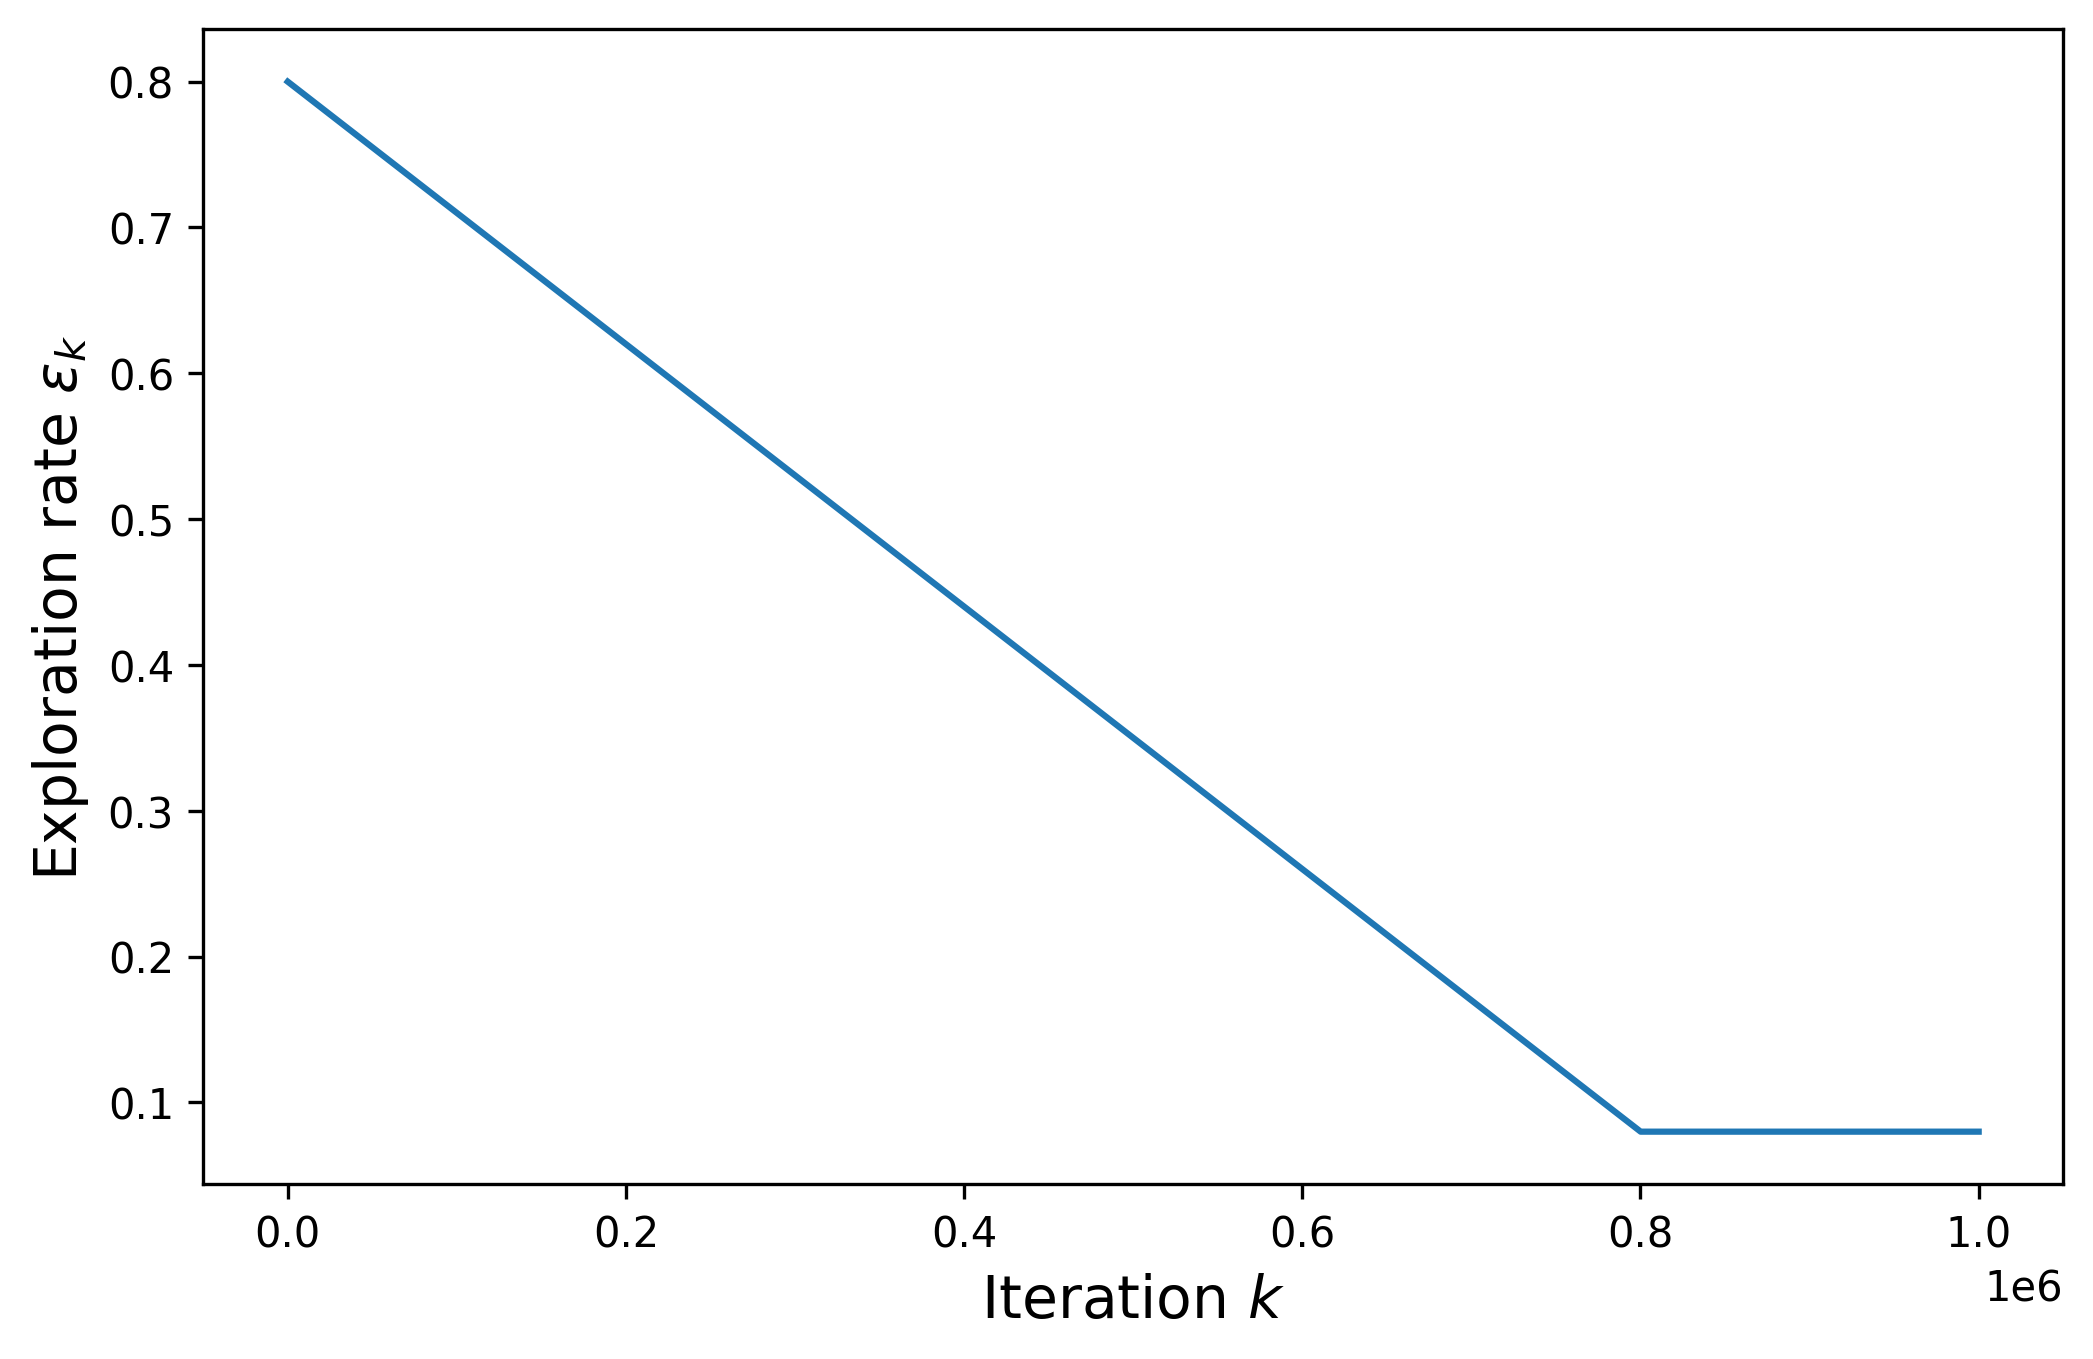
\includegraphics[width=0.75\textwidth]{Plots/FEX/exploration_rate.png}
    \caption{Exploration rate per iteration $k$.}
    \label{fig: DDQN exploration rate}
\end{figure}

Finally, the replay buffer has a capacity of 1'000'000 transitions and, at each iteration, it is filled with $M=1'024$ batches. As such, the buffer is filled up after less than 1'000 iterations. We train the DDQN algorithm on 1'000'000 iterations. Table \ref{tab: DDQN training parameters} gives an overview of parameters used to train the DDQN algorithm.
\begin{table}[h]
    \centering
    \begin{tabular}{rcc}
        \toprule
        & Parameter & Value \\
        \hline
        Number of time steps & $N_t$ & 252 \\
        Number of possible impulses & $N_\zeta$ & 100 \\
        Buffer capacity & $N_\mathcal{D}$ & 1'000'000\\
        Number of batches & $M$ & 1024 \\
        Number of iterations & $N_{\text{iter}}$ & 1'000'000 \\
        Initial spatial value & $x_0$ & $[-2,2]$ \\
        Huber loss truncation & $\delta$ & 1.0 \\
        Minimum exploration rate & $\varepsilon_{\min} $ & 0.08 \\
        Maximum exploration rate & $\varepsilon_{\max}$ & 0.8 \\
        Scaling parameter & $R$ & 2 \\
        Neural network width & $L$ & 4 \\
        Neural network hidden dimensions & $n_\ell$ & $\{2, 512, 64, 101\}$ \\
        Learning rate & lr & 2e-04 \\
        \toprule
    \end{tabular}
    \caption{Parameters used for the training of the DDQN algorithm}
    \label{tab: DDQN training parameters}
\end{table}

\subsection{PPO-SIL}
The PPO-SIL algorithm uses two fully connected feedforward neural networks, one for the decision network and one for the impulse network, with architecture
\begin{equation*}
    \text{Input: }2 \rightarrow 512 \rightarrow 512 \rightarrow 512 \rightarrow 1 \text{: Output}
\end{equation*}
for each network. The input for each of the networks is the timestep $t_n$ and controlled state $X^{(\beta)}$, while the outputs are the decision $d_\chi(t_n,x)$ and impulses $u_\xi(t_n,x)$.

Rewards are computed via the function
\begin{equation*}
    r(t,x,\zeta) = e^{-\delta t} \left(-(x-m)^2 + \gamma w^2 \right) \Delta t + K(t,x,\zeta),
\end{equation*}
where $\zeta \in \mathcal Z$.

The neural networks are trained on Monte Carlo samples of size $N_{\text{rollout}}$ and on a time grid made of $N_t$ time steps over a time horizon of a year. Furthermore, the SIL algorithm's buffer size is 400'000, meaning that 400'000 transitions can be stored. An overview of training parameters used for to train the PPO algorithm can be found in Table \ref{tab: PPO training parameters}.

\begin{table}[h]
    \centering
    \begin{tabular}{rcc}
        \toprule
        & Parameter & Value \\
        \hline
        Number of time steps & $N_t$ & 252 \\
        Number of rollout paths & $N_\text{rollout}$ & 4096 \\
        Number of SIL batches & $N_\text{batch}$ & 4096 \\
        Number of training iterations & $N_\text{iter}$ & 300 \\
        SIL buffer capacity & $N_{\mathcal{B}_\text{good}}$ & 400'000 \\
        SIL loss weight & $\lambda_{\text{SIL}}$ & 0.05 \\
        Entropy regularisation weight & $\lambda_{\mathcal{H}}$ & 1e-03 \\
        Actor loss weight & $\lambda_{\text{actor}}$ & 0.5 \\
        PPO clipping parameter & $\varepsilon$ & 0.3 \\
        Decision network width & $L_{d_\chi}$ & 5 \\
        Decision network hidden dimensions & $n_{d_\chi, \ell}$ & $\{2,512, 512, 512,1\}$ \\
        Impulse network width & $L_{u_\xi}$ & 5 \\
        Impulse network hidden dimensions & $n_{u_\xi, \ell}$ & $\{2,512, 512, 512,1\}$ \\
        Learning rate\footnote{For both decision and impulse networks.} & lr & 2e-04 \\
        Generalised advantage estimate parameter & $\lambda_\text{GAE}$ & 1.0\\
        \toprule
    \end{tabular}
    \caption{Parameters used for the training of the PPO algorithm}
    \label{tab: PPO training parameters}
\end{table}

\section{Results}
For all numerical results found in this section, we use the parameter values reported in Table \ref{tab: FEX rate params}. We perform a convergence test on the explicit-impulse scheme to validate that the numerical scheme indeed converges to a solution as the numerical grid is refined. The DDQN and PPO algorithm are trained using the hyperparameters found in Tables \ref{tab: DDQN training parameters} and \ref{tab: PPO training parameters}, respectively, and are compared against the explicit-impulse control scheme. All numerical experiments were implemented on the same computer, specifically on a MacBook Pro M2, with 10 CPU and 10 GPU cores, and 16GB of unified RAM. 

\subsection{Explicit-impulse scheme and convergence test}
Figure \ref{fig: explicit impulse 2D plot} shows the numerical approximation $V$ of the value function at time $t=0$. The numerical grid used for the approximation consists of $N_t=252$, $N_x=401$, and $N_\zeta=101$ points. The numerical solution has a curved profile near the target $m$, which corresponds to the continuation region where no impulses are applied. However, if the state $x$ moves sufficiently far from $m$, the value becomes approximately affine due to interventions and the corresponding affine transaction costs. A kink can therefore be observed the boundary of between both regions, where the curved part meets the affine tails.
\begin{figure}[H]
    \centering
    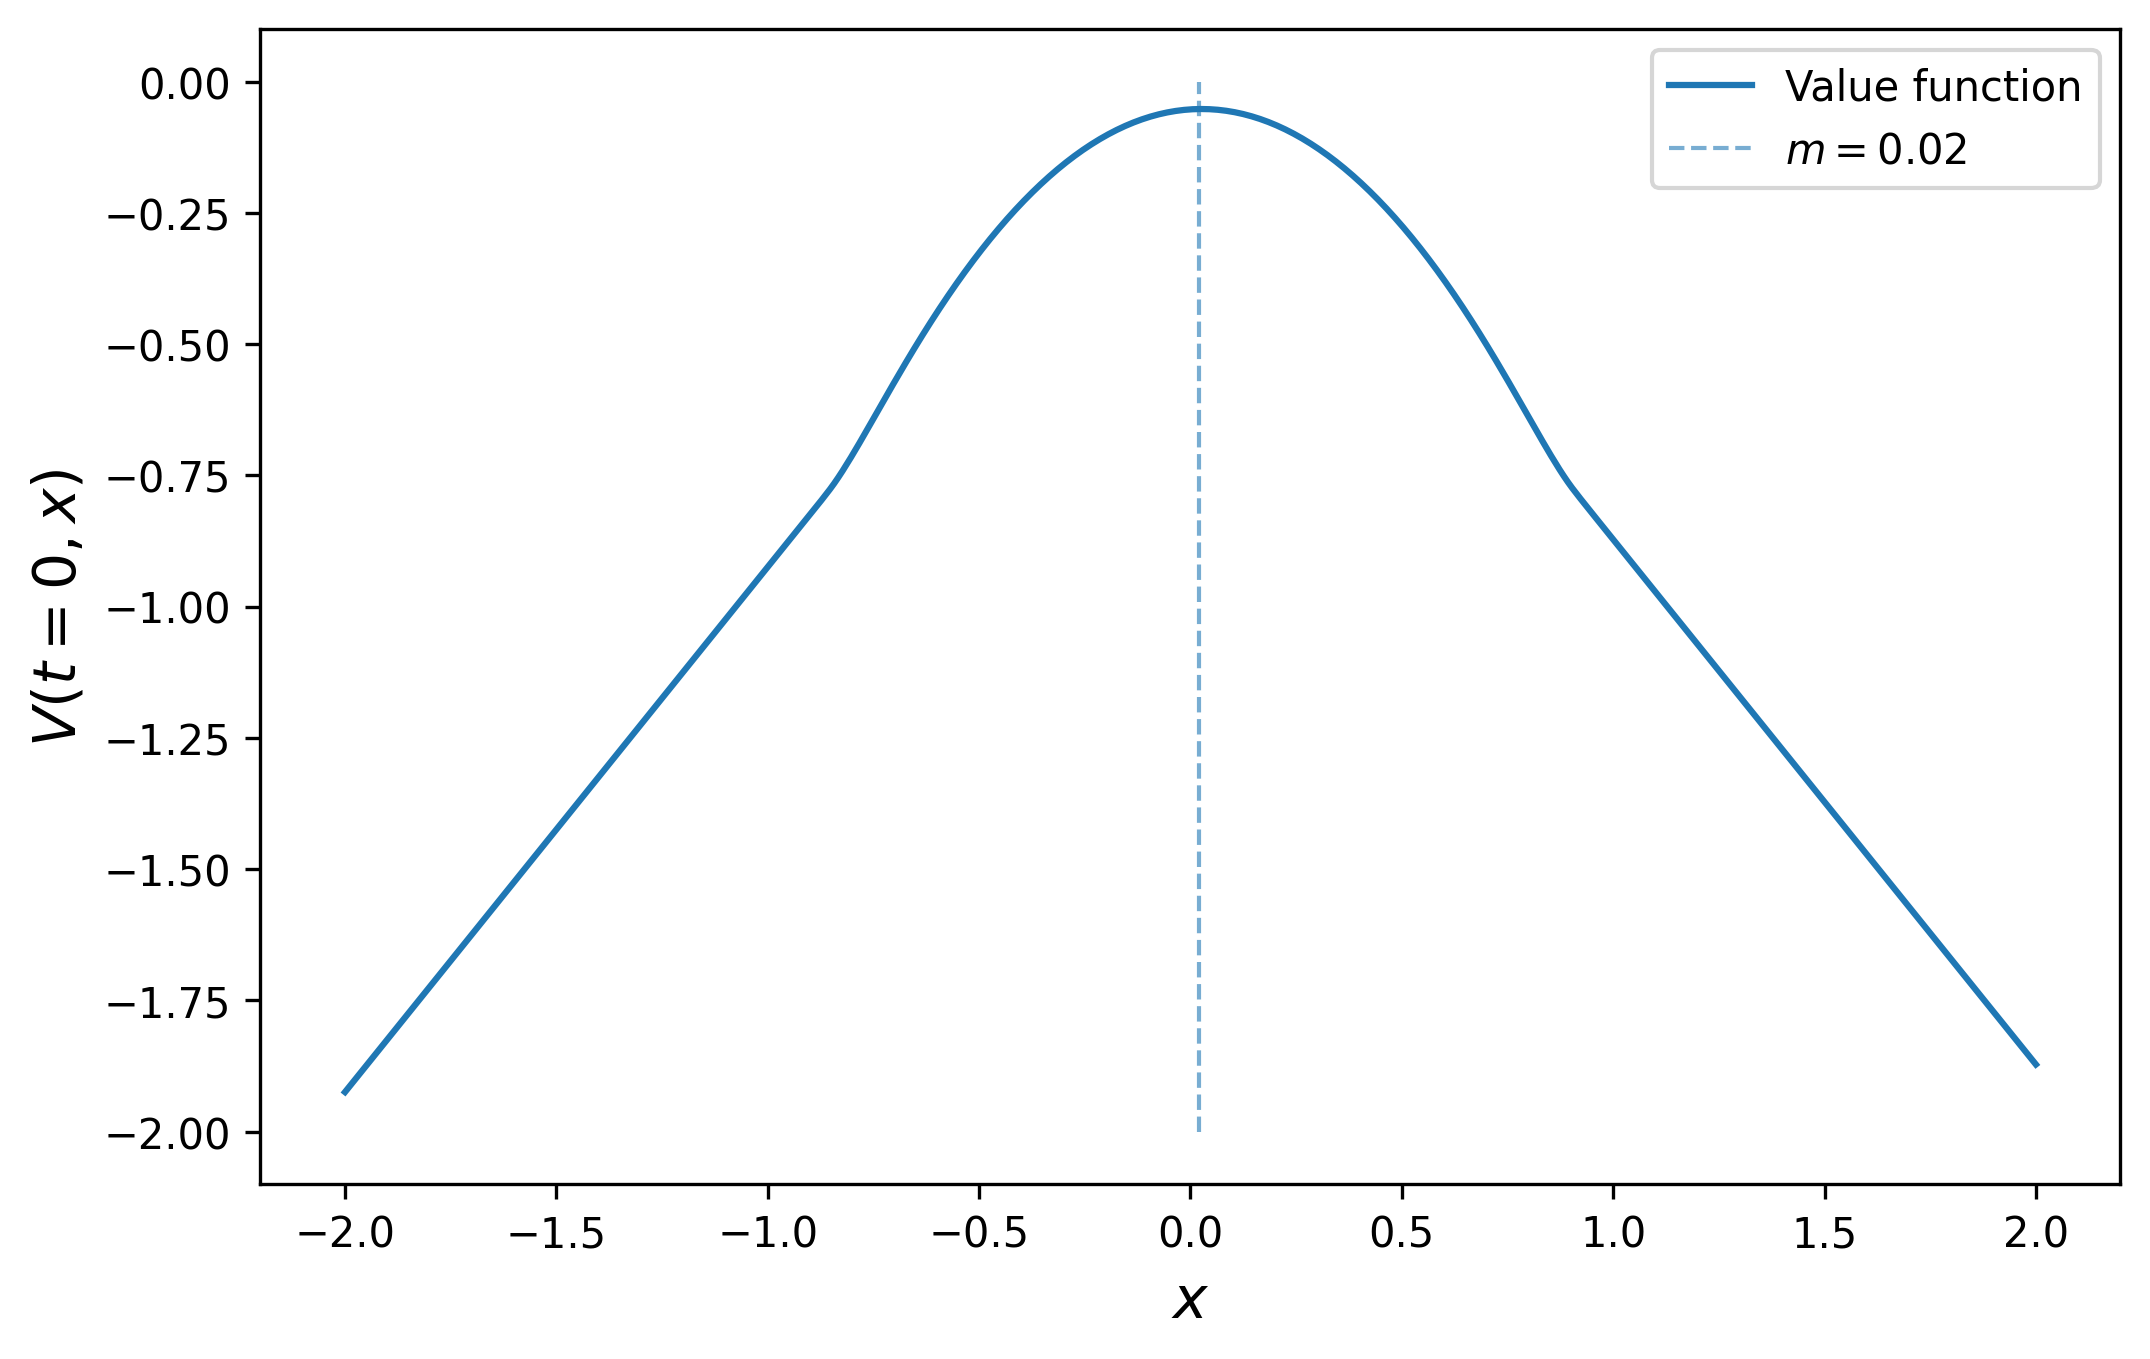
\includegraphics[width=0.75\textwidth]{Plots/FEX/explicit_impulse_2D.png}
    \caption{Numerical solution of FEX rate problem at time $t=0$.}
    \label{fig: explicit impulse 2D plot}
\end{figure}

Figure \ref{fig: explicit impulse 3D plot} shows the behaviour of the value function across time. Similarly to the results shown in \ref{fig: explicit impulse 2D plot}, the value function approximation across time is curved around the target $m$, which corresponds to the continuation region, while for sufficiently large deviations from $m$, the value becomes approximately affine in $x$, corresponding to intervention. As $t$ approaches the terminal time, the value function moves towards the terminal condition $g\equiv 0$, reflecting that fewer future running costs remain to be accumulated.
\begin{figure}[h]
    \centering
    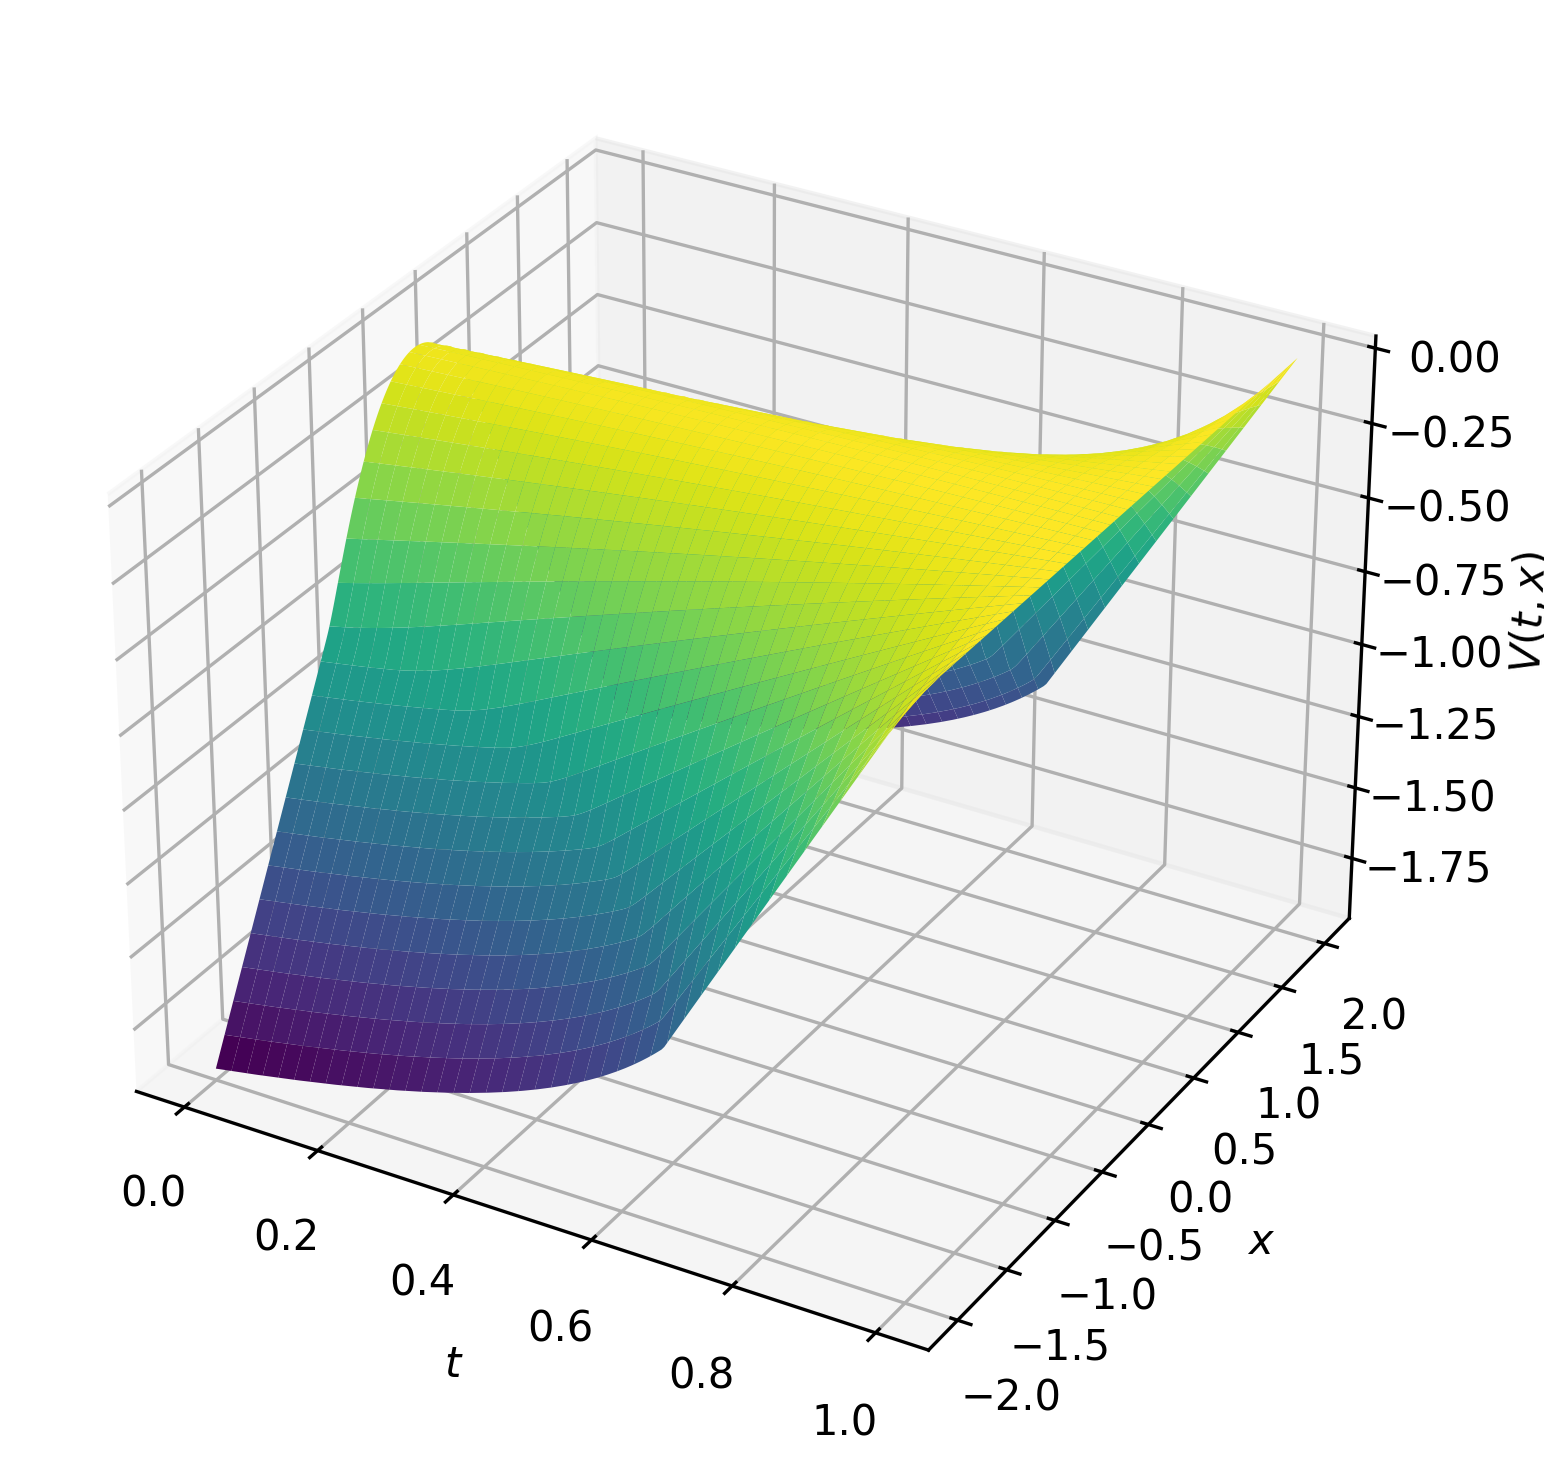
\includegraphics[width=0.6\textwidth]{Plots/FEX/explicit_impulse_3D.png}
    \caption{Numerical solution of FEX rate problem at for times $t \in [0,1]$.}
    \label{fig: explicit impulse 3D plot}
\end{figure}

Table \ref{tab: impulse control convergence test} presents the approximations of the value function at $t=0$ and $x=m$ obtained using the explicit‑impulse scheme under successive grid refinements. The corresponding numbers of time, spatial, and impulse size discretisation points, denoted by $N_t$, $N_x$, and $N_\zeta$ respectively, are also reported. The values stabilise around $V(0,m) \approx -0.05129$, showing empirical convergence.
\begin{table}[h]
    \centering
    \begin{tabular}{cccccc}
        \toprule
        $N_t$ & $N_x$ & $N_\zeta$ & $V(t=0, x=m)$ & Ratio & CPU time (s) \\
        \hline
        16 & 32 & 16 & -0.057488 & & 2.63e-03 \\
        32 & 64 & 32 & -0.054501 & & 2.68e-03 \\
        64 & 128 & 64 & -0.052996 & 1.99 & 5.17e-03 \\
        128 & 256 & 128 & -0.052377 & 2.43 & 1.67e-02 \\
        256 & 512 & 256 & -0.052120 & 2.41 & 1.05e-01 \\
        512 & 1024 & 512 & -0.051995 & 2.06 & 1.67e+00 \\
        1024 & 2048 & 1024 & -0.051938 & 2.19 & 1.08e+01 \\
        \bottomrule
    \end{tabular}
    \caption{Convergence test for the explicit-impulse scheme}
    \label{tab: impulse control convergence test}
\end{table}

Because the convergence test shows stable approximation results, and since the computed value
function exhibits the expected continuation and intervention structure, we may apply the explicit-impulse scheme as a benchmark for comparison against the aforementioned DRL algorithms.

\subsection{DDQN approximation}
Consider Figure \ref{fig: DDQN vs FD 2D plot}, where the DDQN and explicit-impulse schemes are compared for time $t=0$ and $x \in [-2,2]$. As one can observe, the DDQN algorithm reproduces a value function approximation comparable to the benchmark. In particular, the DRL algorithm is able to approximate the value function near the target $m$ with a curve, while the part where the value function transitions from a curve to the affine tails is also captured by the DRL algorithm. Furthermore, the agreement between both schemes is strongest in the central part of the domain, where the value function is smooth and where the simulated training data are more concentrated. The learned value function also captures the kinks at the boundary between the continuation and intervention regions, albeit not as precisely as the finite-difference scheme. In general, the DDQN is able to learn both the shape of the value function and the impulse controls required for different values for the log-FEX rate $x$. 

When it comes to the separations between both approximations in Figure \ref{fig: DDQN vs FD 2D plot}, largest errors happen around the (non-differentiable) kink. This is in part because the DDQN curve shown in the aforementioned figure is obtained by greedy impulse selection \eqref{eqn: DDQN greedy impulse choice} and Monte Carlo approximation. Specifically, if neighbouring impulses yield similar values on the free boundary, the maximisation step in \eqref{eqn: DDQN greedy impulse choice} chooses the impulse with the largest implied value estimate, so that small errors may yield suboptimal impulses. As a consequence, small perturbations in the learned value function may lead to different selected impulses, which lead to small
local irregularities in the plotted approximation.

\begin{figure}[h]
    \centering
    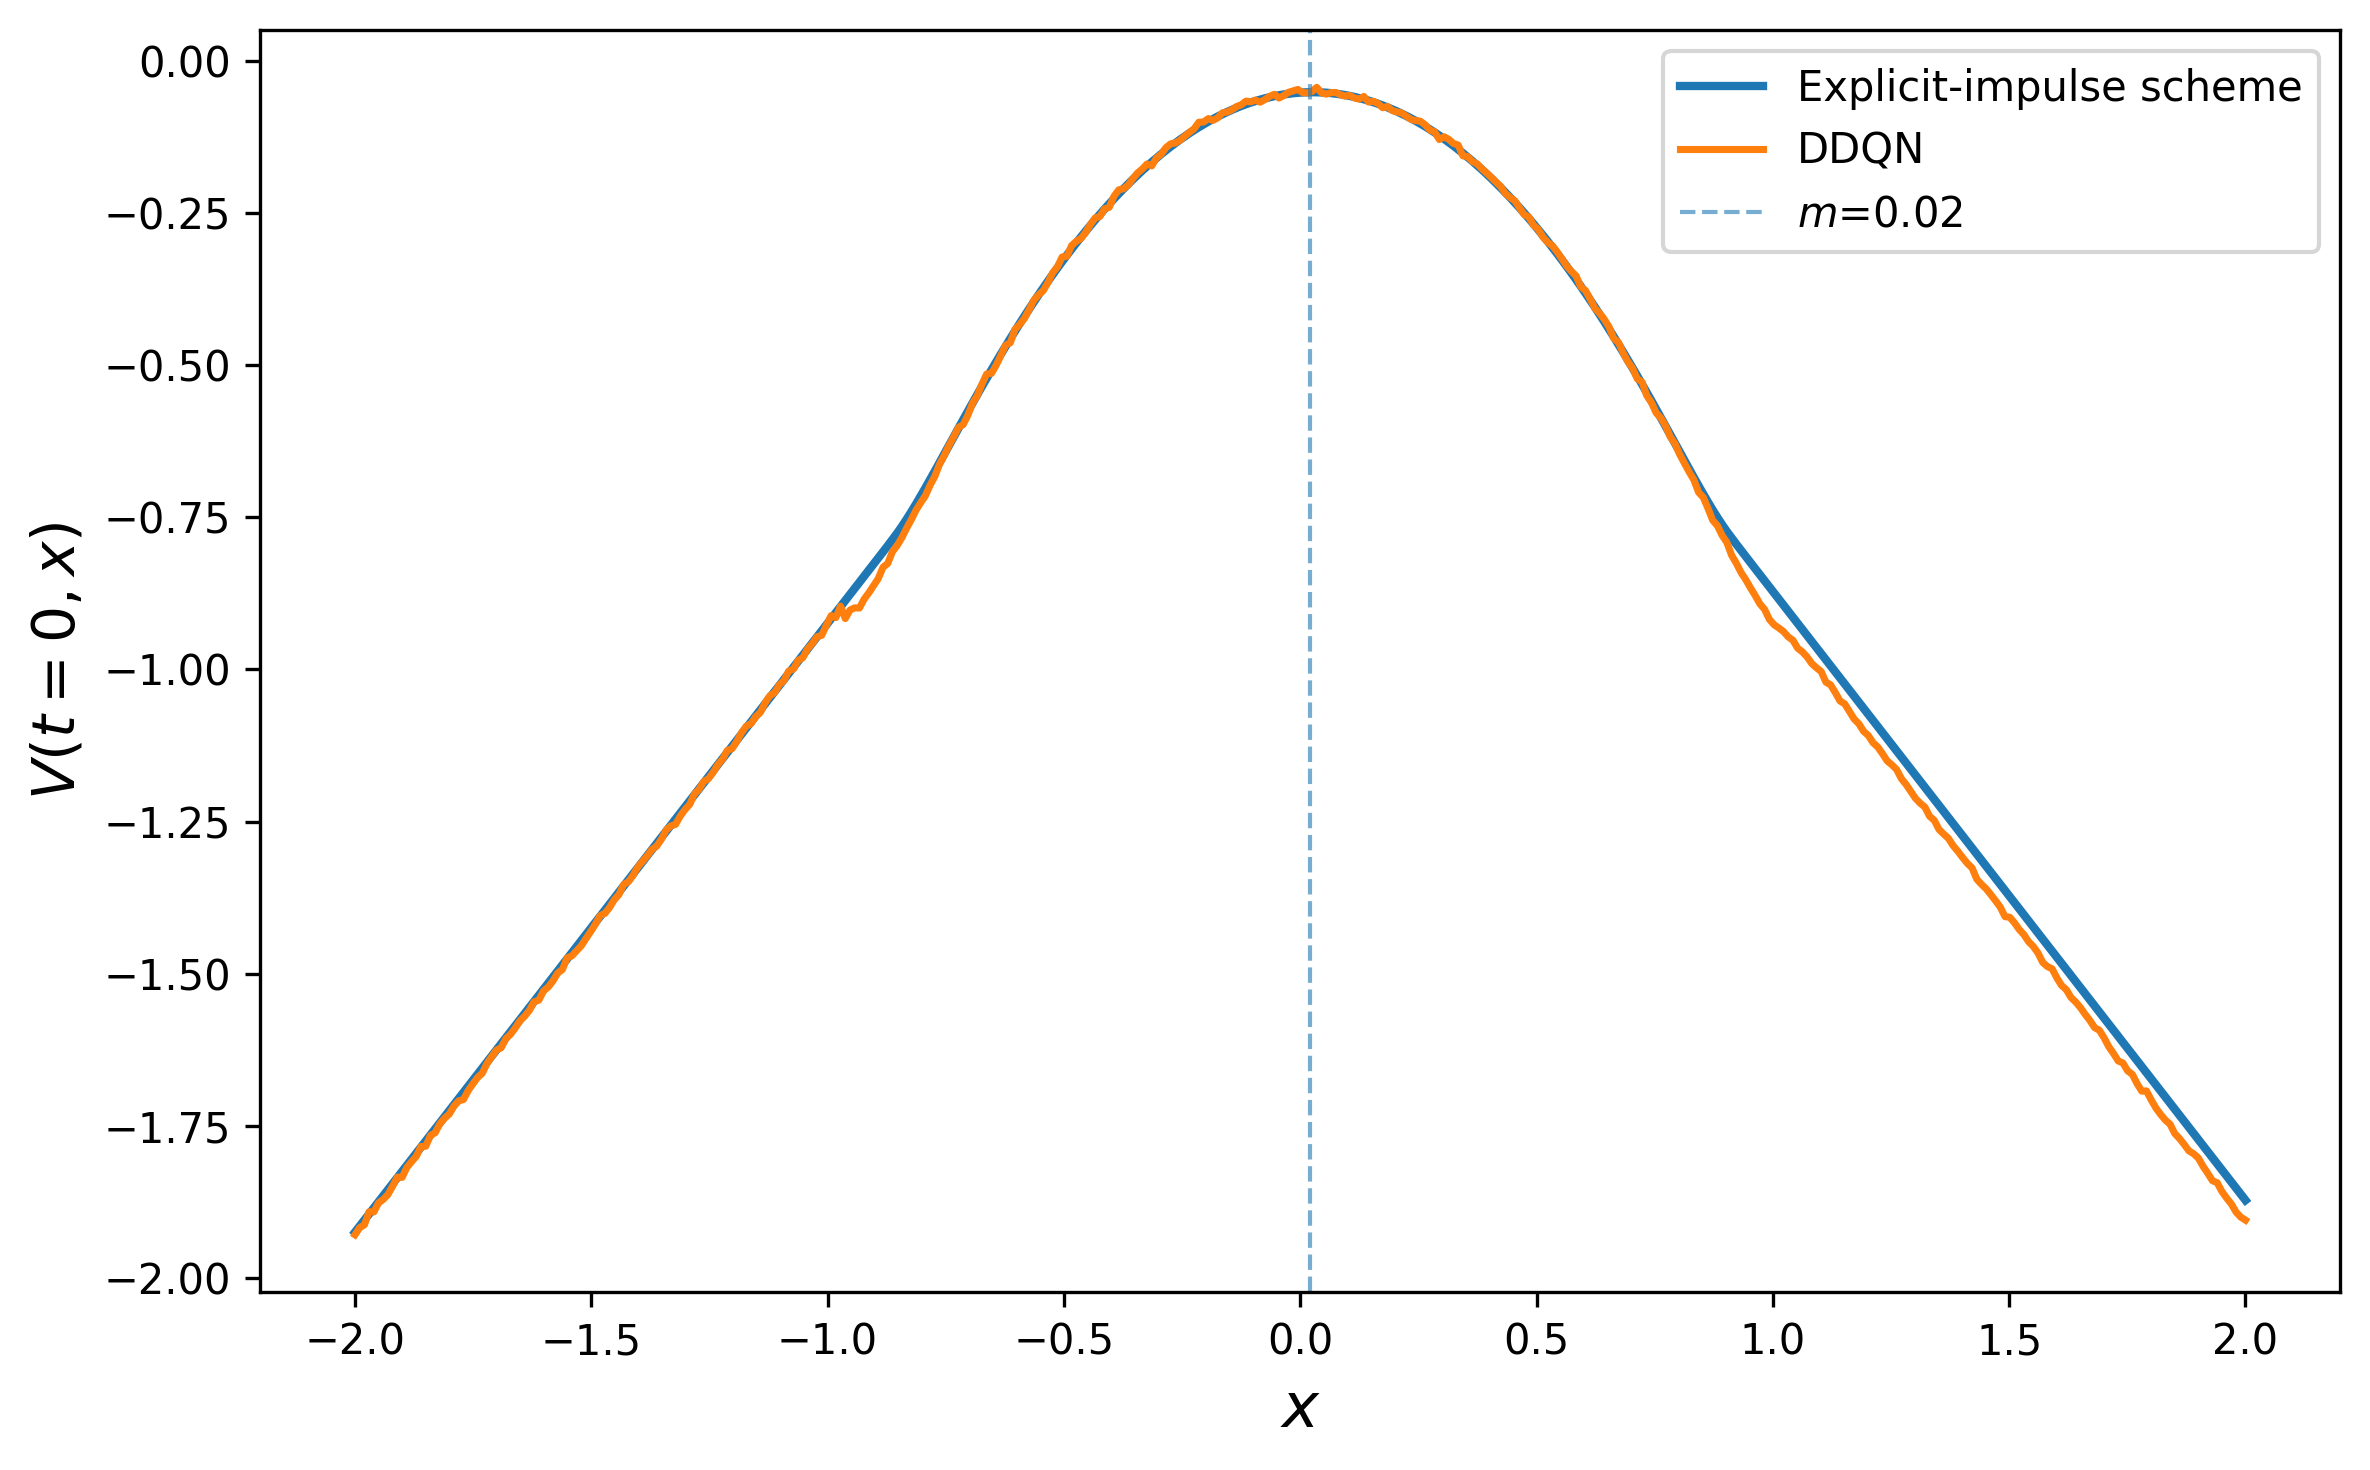
\includegraphics[width=0.75\textwidth]{Plots/FEX/DDQNvsFD_2D.png}
    \caption{Comparison of DDQN and Explicit-impulse scheme value function approximations}
    \label{fig: DDQN vs FD 2D plot}
\end{figure}

Figure \ref{fig: DDQN vs FD 3D plot} gives the corresponding comparison over the time interval $t \in [0,T]$. We observe that the DDQN surface approximation is qualitatively close to the explicit-impulse surface, and that the DDQN surface moves towards the terminal condition $g \equiv 0$ as $t$ approaches $T$. This indicates that the DDQN approximation captures the time-dependent structure of the value function, including the evolution of the intervention and continuation regions. When compared to the explicit-impulse scheme, the largest visible deviations seem to occur close to the free boundary and in regions that are less frequently visited during simulation. The regions that are visited less frequently are those in which $x$ takes large positive values since the negative drift in \eqref{eqn: FEX problem controlled X c} reduces the likelihood that the stochastic process $X$ takes positive values as time goes by.

\begin{figure}[h]
    \centering
    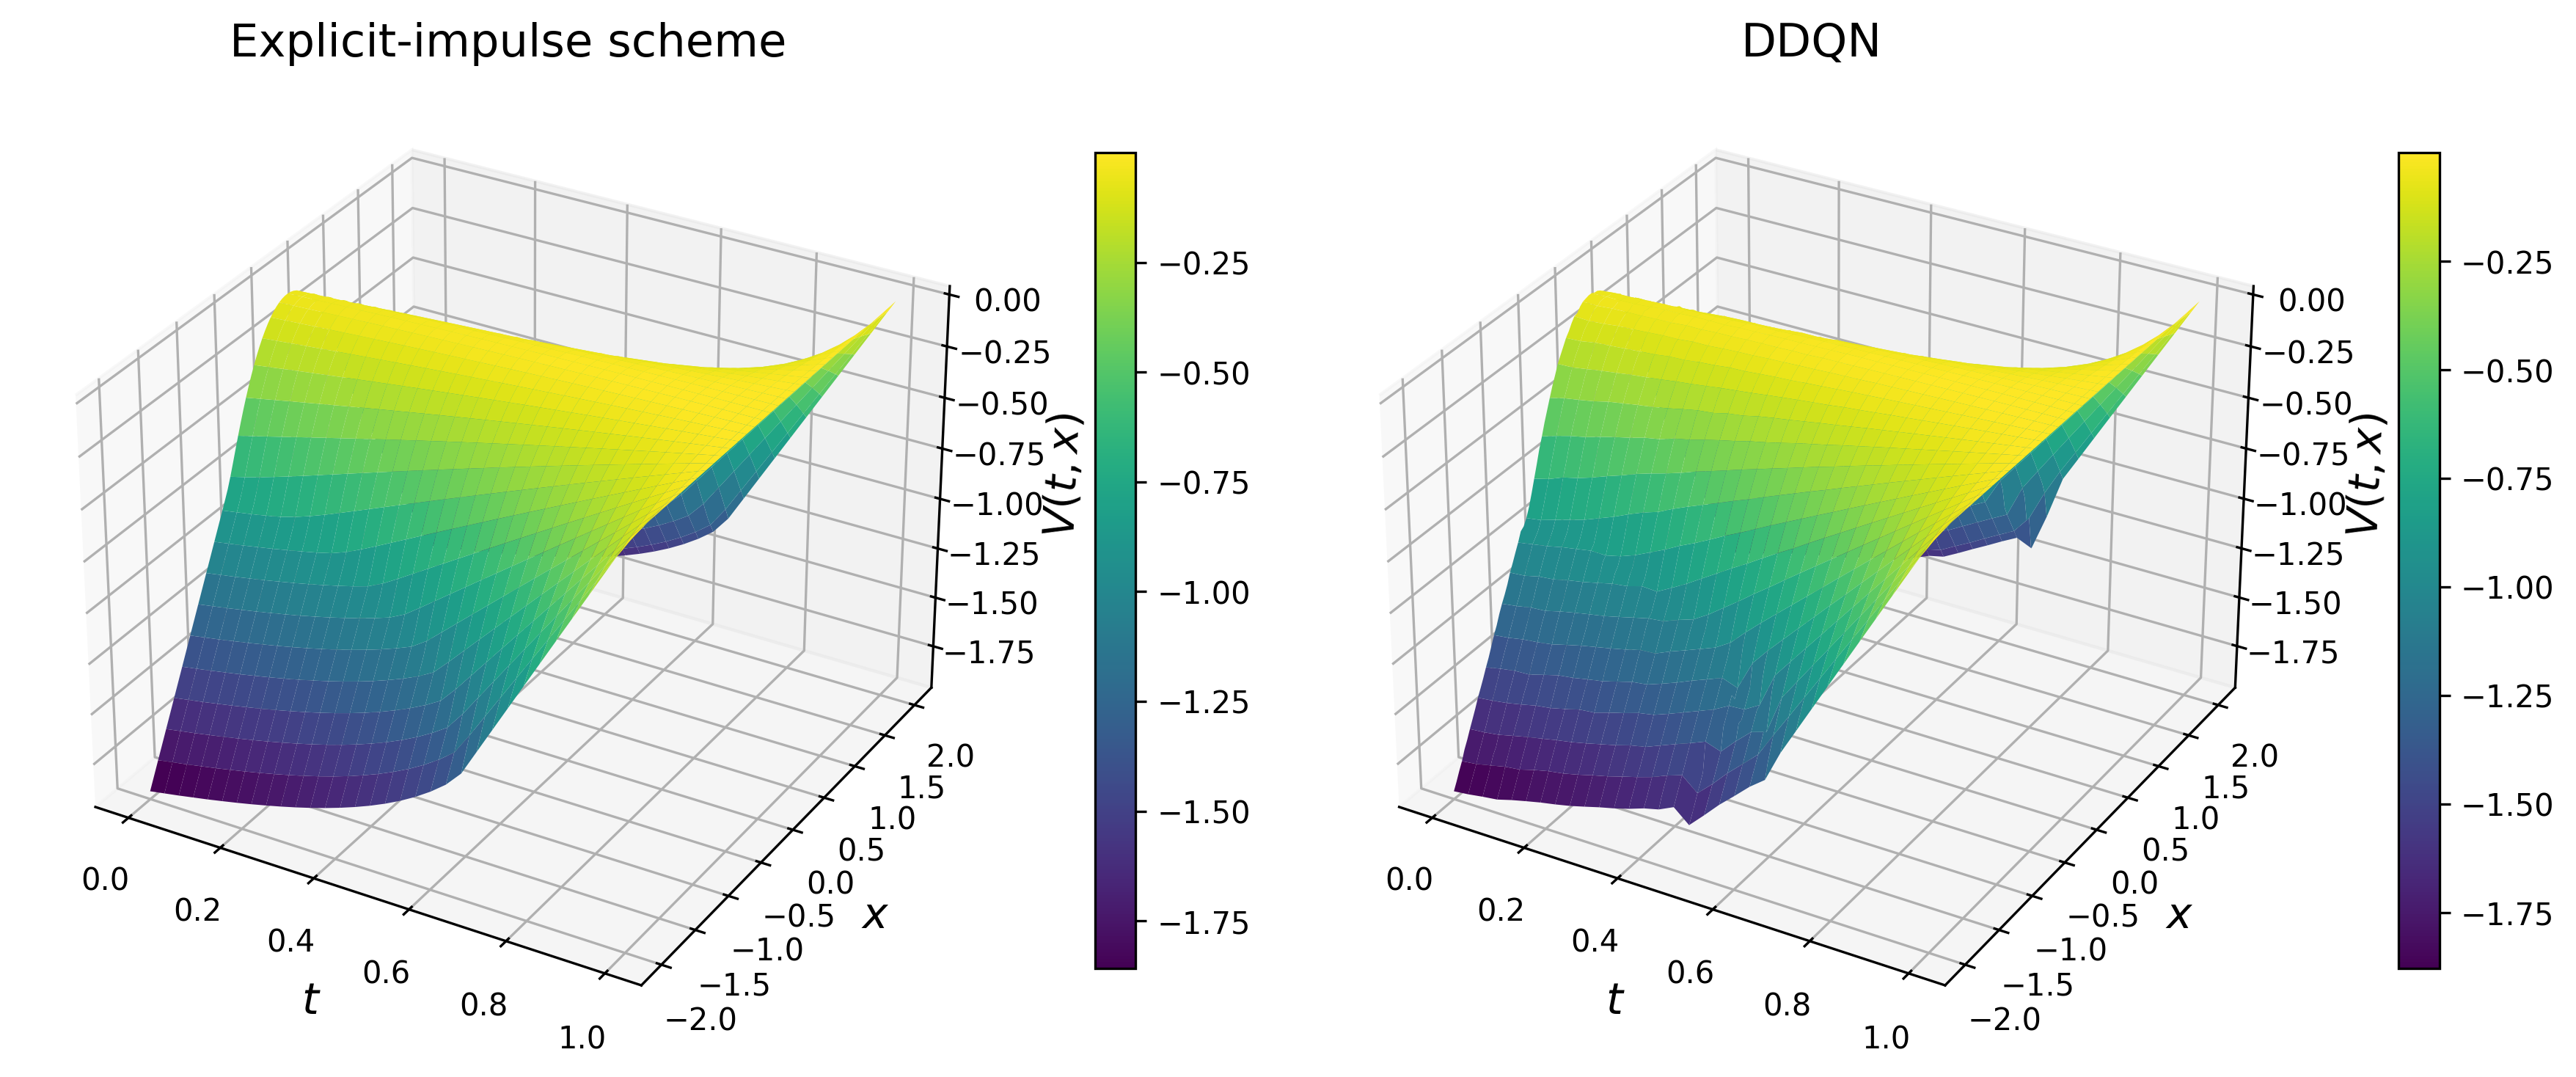
\includegraphics[width=\textwidth]{Plots/FEX/DDQNvsFD_3D.png}
    \caption{Comparison of DDQN and Explicit-impulse scheme value function approximations for times $t \in [0,1]$.}
    \label{fig: DDQN vs FD 3D plot}
\end{figure}

Figure \ref{fig: DDQN vs FD error plot} shows the pointwise error between the DDQN approximation and the explicit-impulse benchmark. The heatmap confirms that the error is small over most of the computational domain. The largest errors can be found near the free boundary, where the value function transitions between the continuation and intervention regimes. This is also the region where the impulse decision is the most sensitive. Hence, a small error in the learned value function can change whether the greedy policy selects intervention or continuation. The resulting error heatmap is therefore useful for understanding what free boundary the network learned.

\begin{figure}[h]
    \centering
    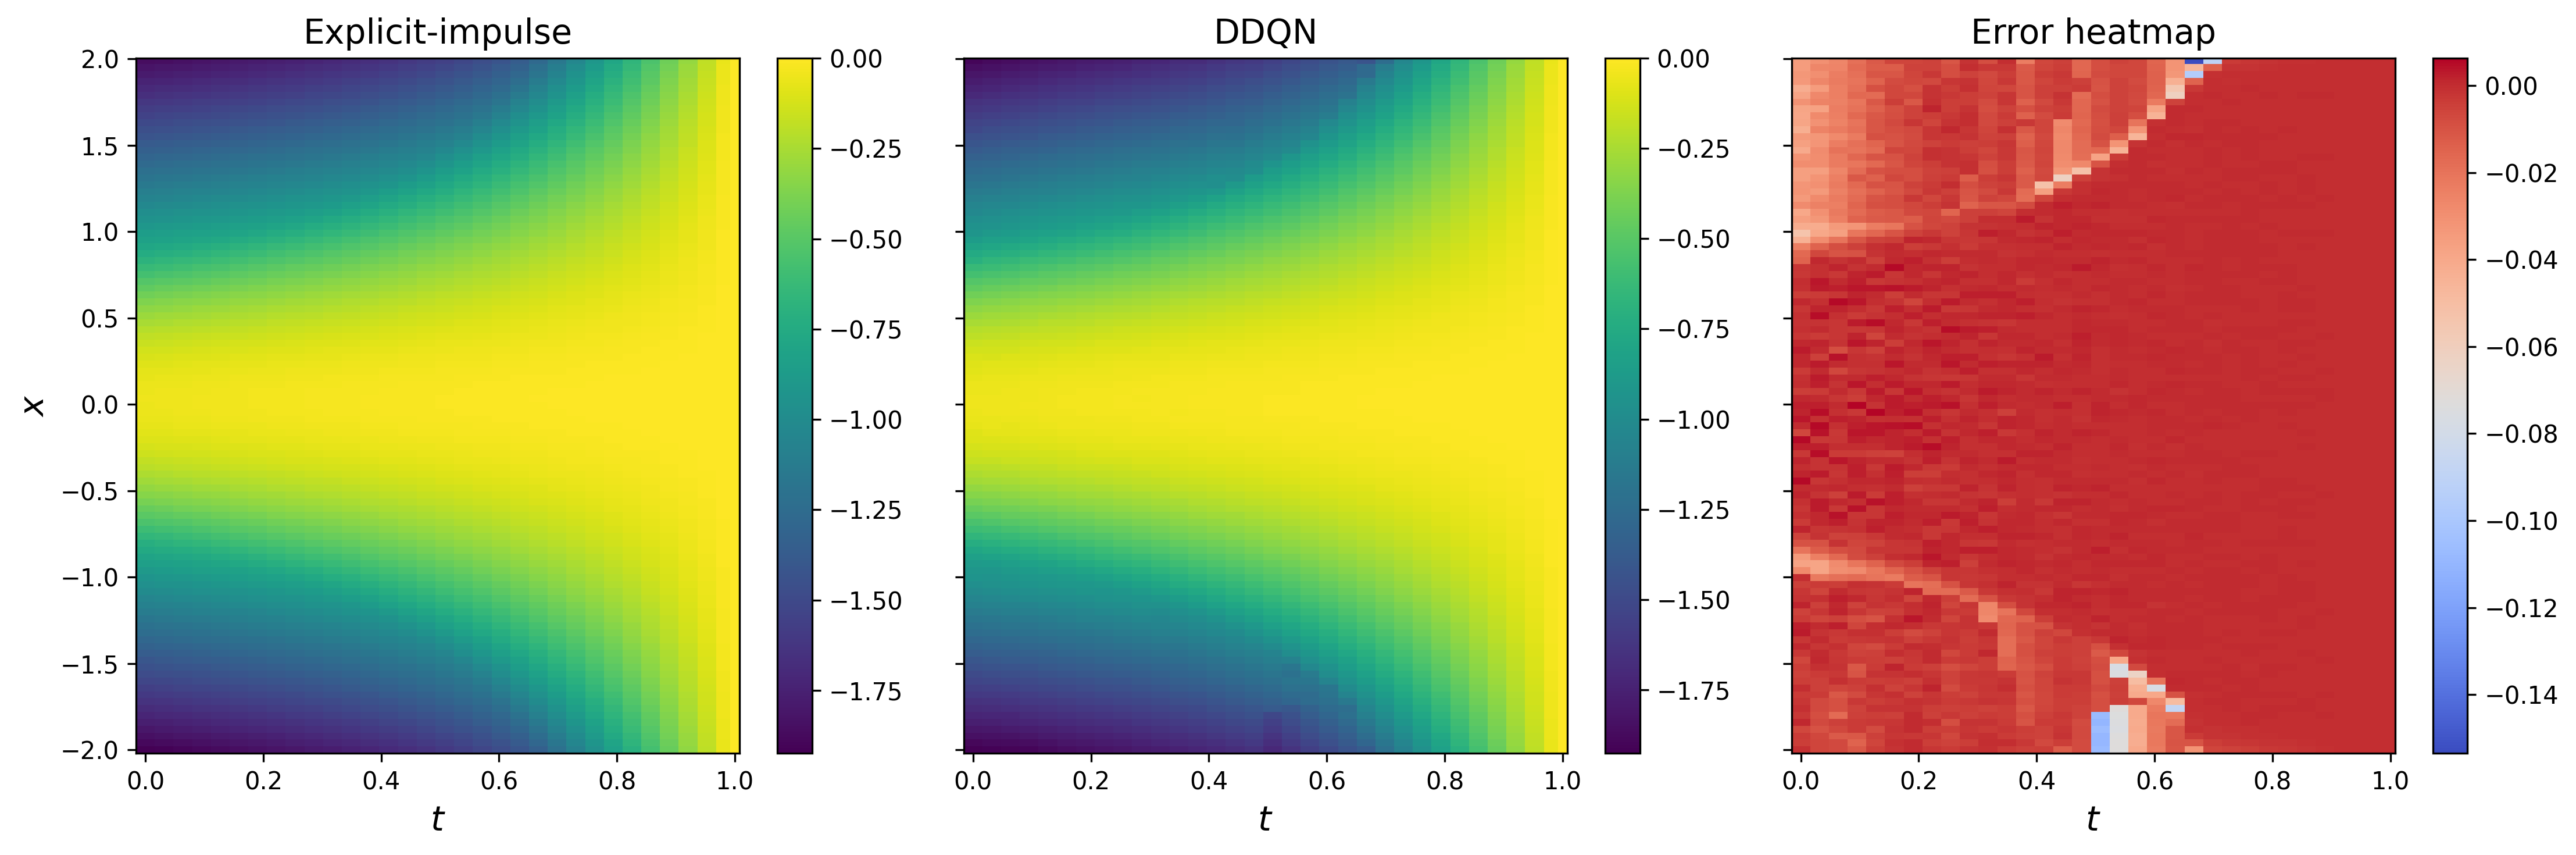
\includegraphics[width=\textwidth]{Plots/FEX/DDQN_Error_heatmap.png}
    \caption{Error heatmap of the DDQN algorithm}
    \label{fig: DDQN vs FD error plot}
\end{figure}

Besides the numerical accuracy, another important aspect to consider is the computation cost, which in our case differs substantially between the two methods. The DDQN training time was approximately 122 minutes, whereas the explicit-impulse scheme only needed 36.6 ms to compute the value function. Another aspect worth mentioning is the training stability of the DDQN algorithm. As the algorithm involves a large number of hyperparameters, the set of possible configurations is extensive. In practice, we therefore selected the first set of hyperparameters that produced satisfactory results, although further tuning could lead to improvements in performance and computational efficiency. We also observe that the DDQN algorithm is highly sensitive to these choices, as even small changes in hyperparameters can result in significantly worse performance.

Overall, the DDQN approximation is consistent with the explicit-impulse benchmark. The algorithm is able to reproduce the continuation region, the affine intervention tails, the time evolution of the surface, and the approximate location of the free boundary. Although the DDQN is substantially more expensive to train and exhibits larger errors near the boundary and in under-sampled regions, both methods show similar results. The DDQN algorithm can therefore be seen as an alternative approach for the approximation of value functions.

\subsection{PPO-SIL approximation}
Figure \ref{fig: PPO vs FD 2D plot} compares the approximation at $t=0$ and for $x \in [-2,2]$. At the first glance, the PPO-SIL algorithm's value function approximation is comparable to the benchmark. Indeed, the agreement between both schemes is particularly strong around the target level $m$, where the value function is smooth, and path simulations of the log-FEX rate provide relatively informative training data. In addition, the figure indicates that the learned policy can effectively capture the intervention structure of the problem, as the value function stays relatively close to the explicit-impulse approximation, with small errors present near the intervention boundary.

\begin{figure}[h]
    \centering
    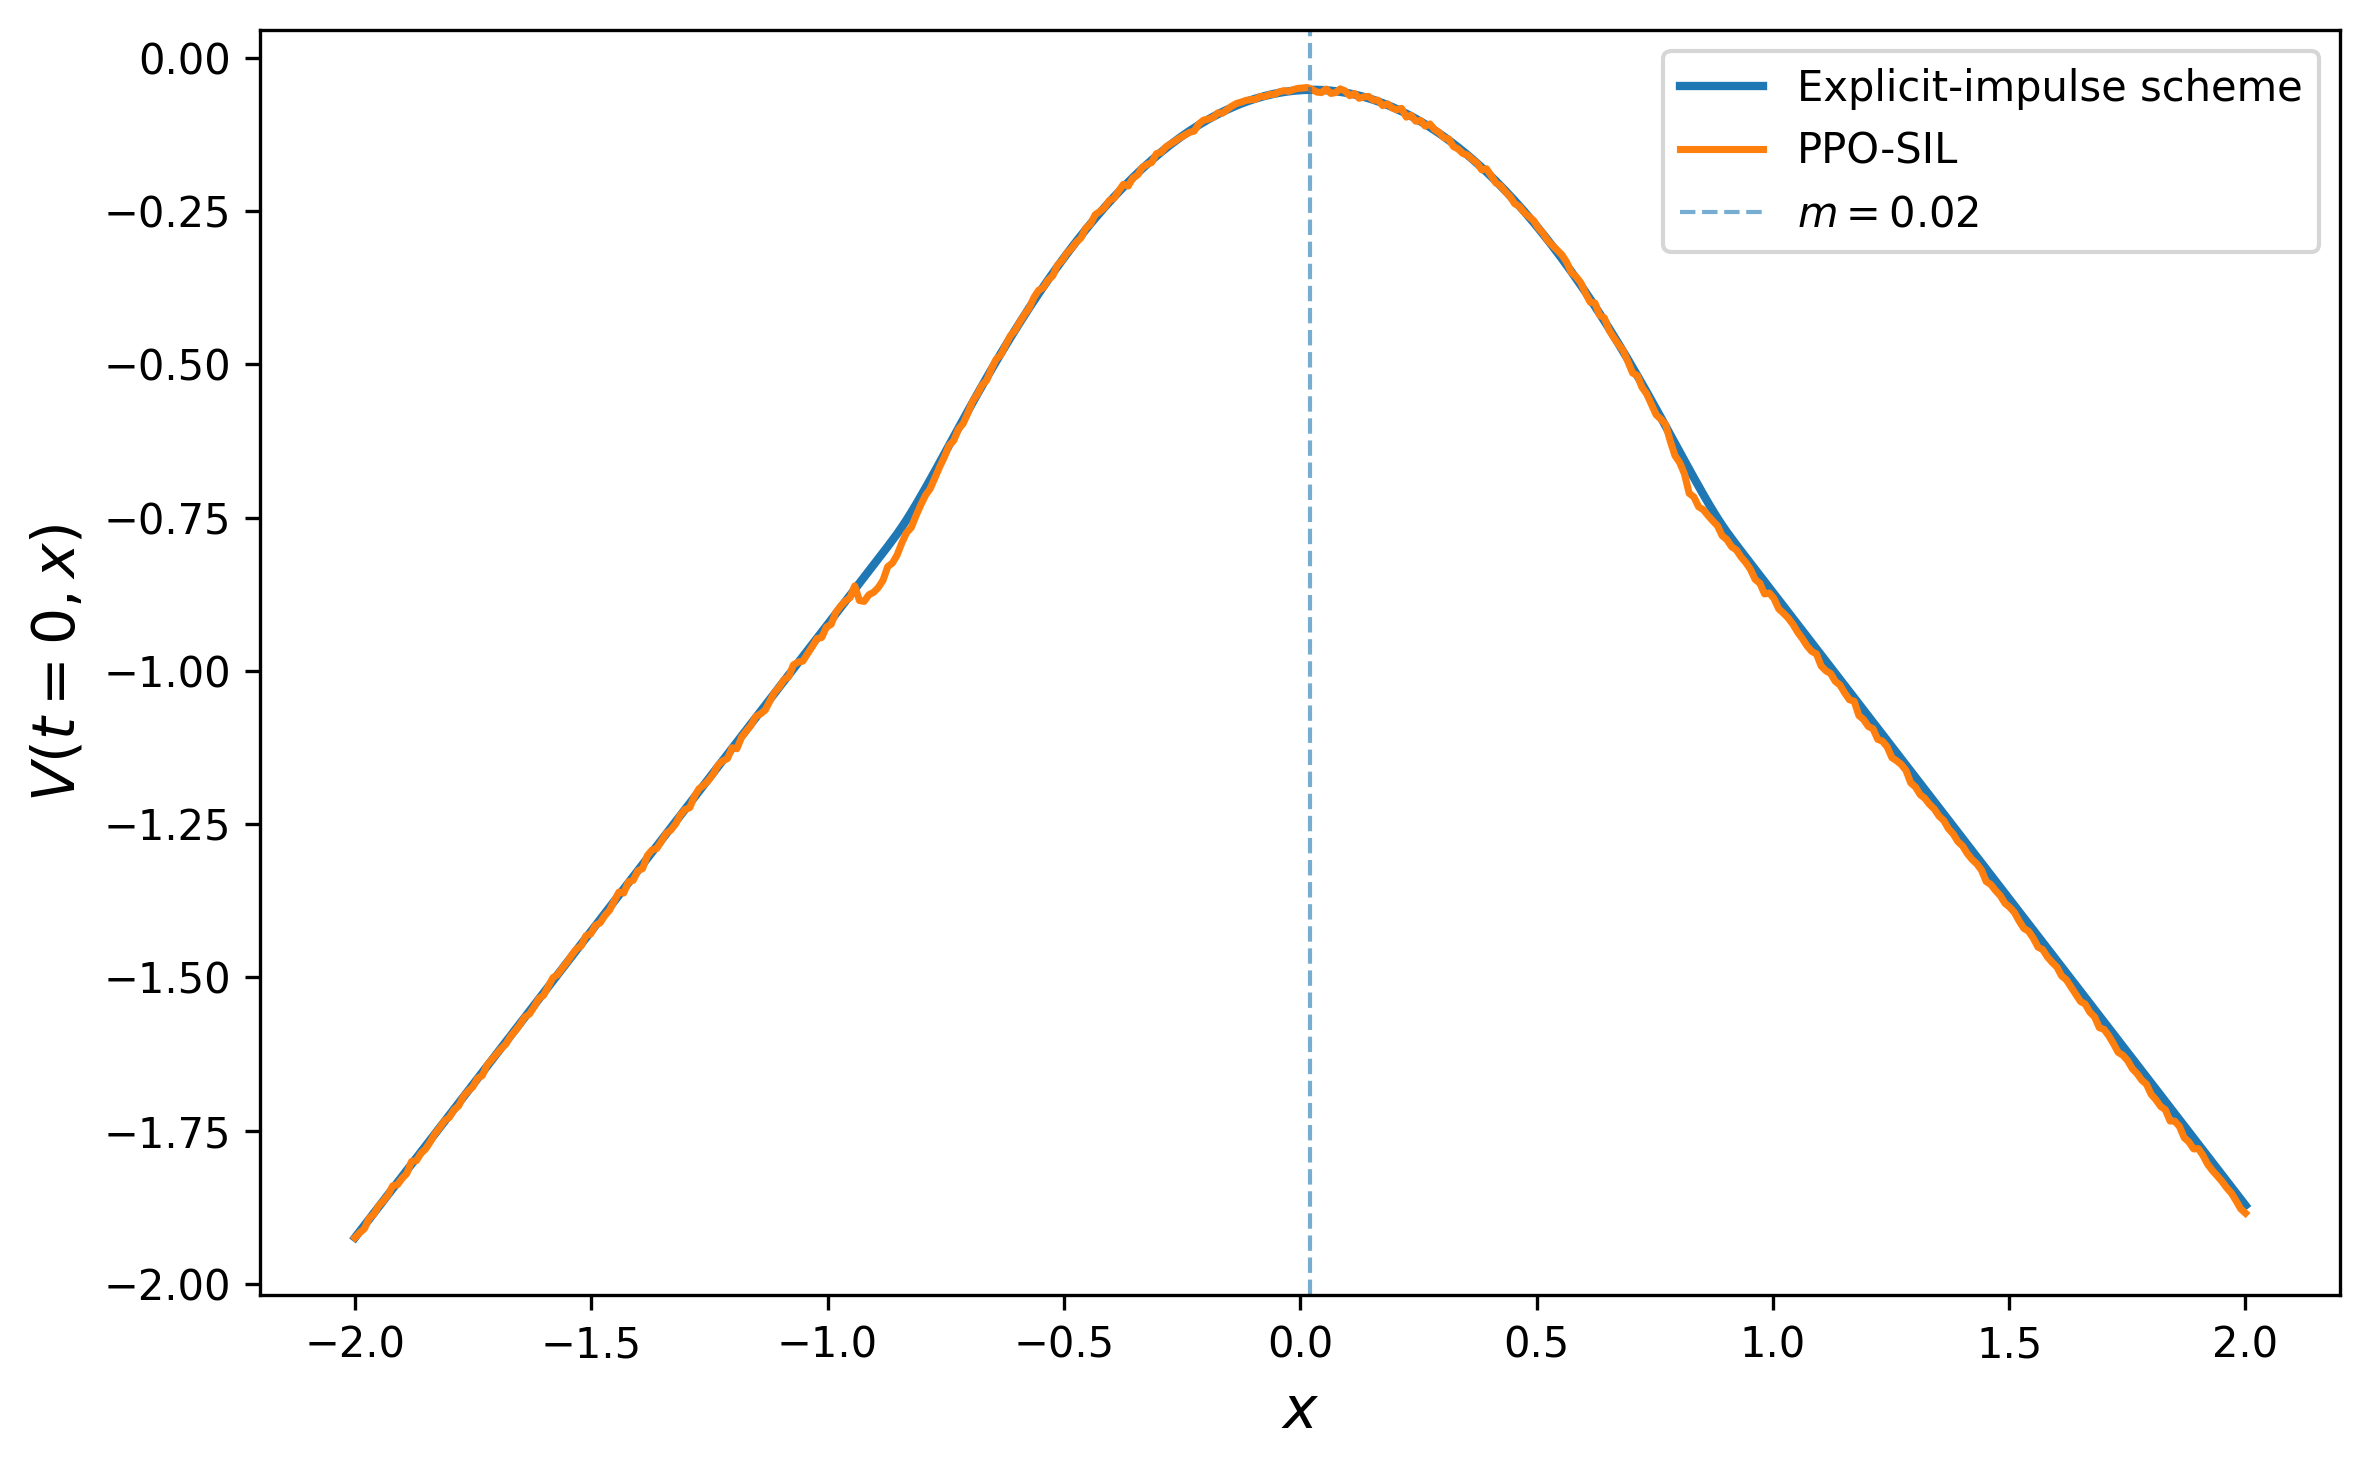
\includegraphics[width=0.75\textwidth]{Plots/FEX/PPOvsFD_2D.png}
    \caption{Comparison of PPO-SIL and explicit-impulse scheme value function approximations}
    \label{fig: PPO vs FD 2D plot}
\end{figure}

Figure \ref{fig: PPO vs FD 3D plot} compares the approximation of the surfaces of the value functions of both schemes over the time interval $t \in [0,1]$. The PPO-SIL surface reproduces the main qualitative structure of the explicit-impulse scheme, with the value being largest near the target $m$ and the tails being approximately affine in $x$. The surface moves towards the terminal condition as $t$ approaches 1. Thus, the PPO-SIL has learned the broad time-dependent continuation structure of the impulse-control problem. 

However, the PPO-SIL approximation still has errors, which appear mostly in the outer regions, especially for positive $x$-values and later times. These errors are most likely caused by the combination of simulation-based training and under-sampling of parts of the state space. In particular, the FEX process has a negative drift in this experiment, meaning that simulated paths tend to move towards negative $x$-values. Consequently, the algorithm observes fewer samples with positive $x$-values, making the approximation less reliable in that part of the domain. 

\begin{figure}[h]
    \centering
    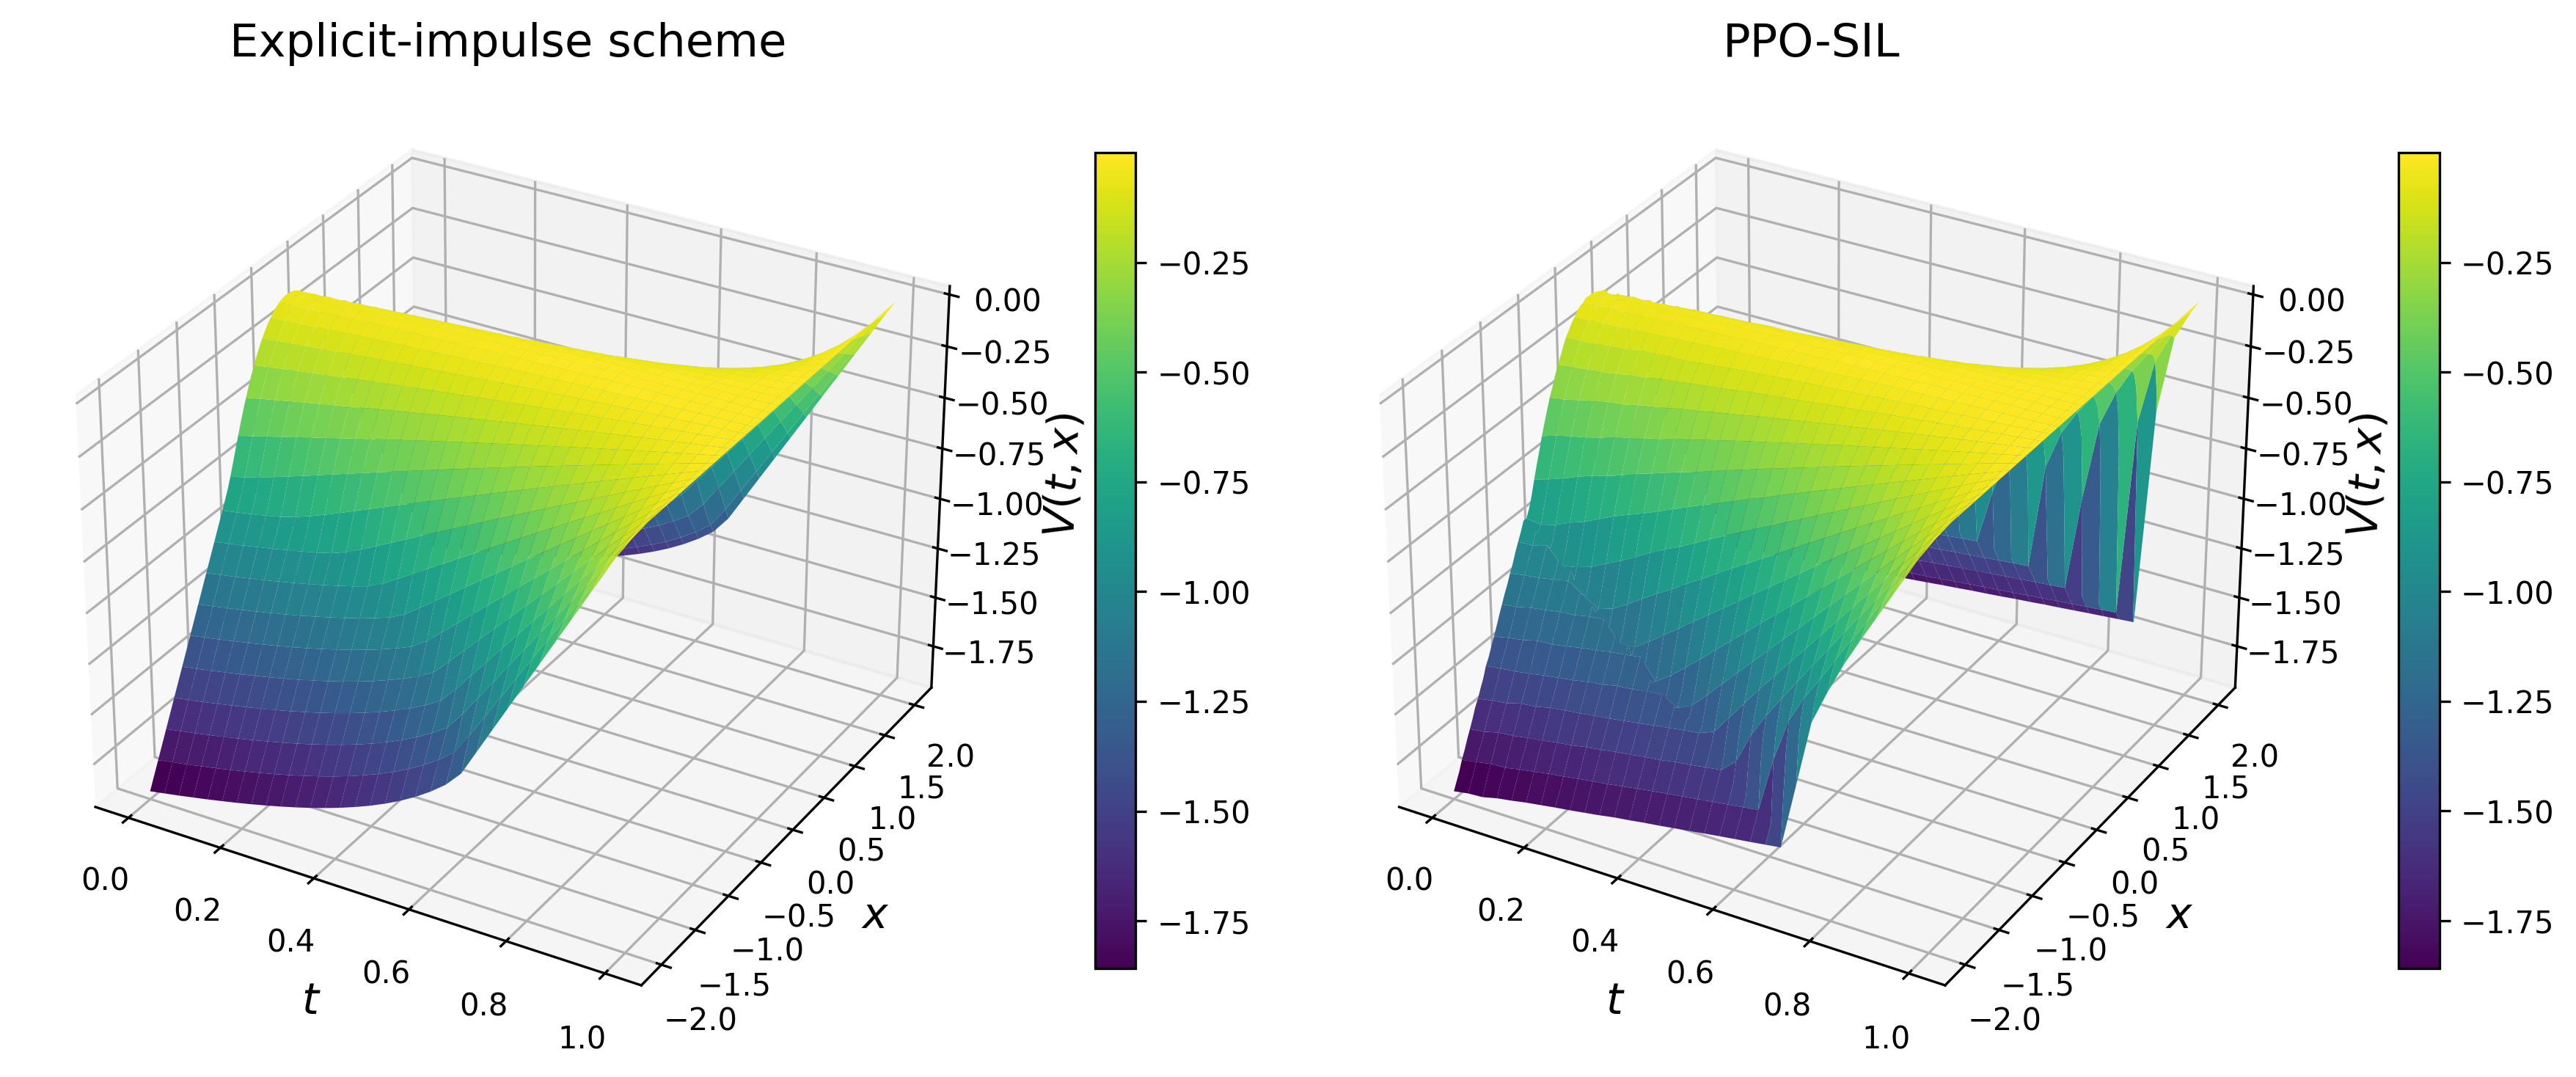
\includegraphics[width=\textwidth]{Plots/FEX/PPOvsFD_3D.png}
    \caption{Comparison of PPO-SIL and Explicit-impulse scheme value function approximations for times $t \in [0,1]$}
    \label{fig: PPO vs FD 3D plot}
\end{figure}

This observation is further supported by the error plot in Figure \ref{fig: PPO vs FD error plot}. Although errors are small for most of the computational domain, especially in the central region around the target, the largest errors can be found in the under-sampled positive $x$ region, as well as near the boundary of the continuation and intervention regions. Moreover, we observe that the learned policy tends to wait rather than intervene immediately, acting only once the boundary becomes more clearly defined. This behavior may possibly explain why the policy learns an almost linear boundary between the continuation and intervention regions.

\begin{figure}[H]
    \centering
    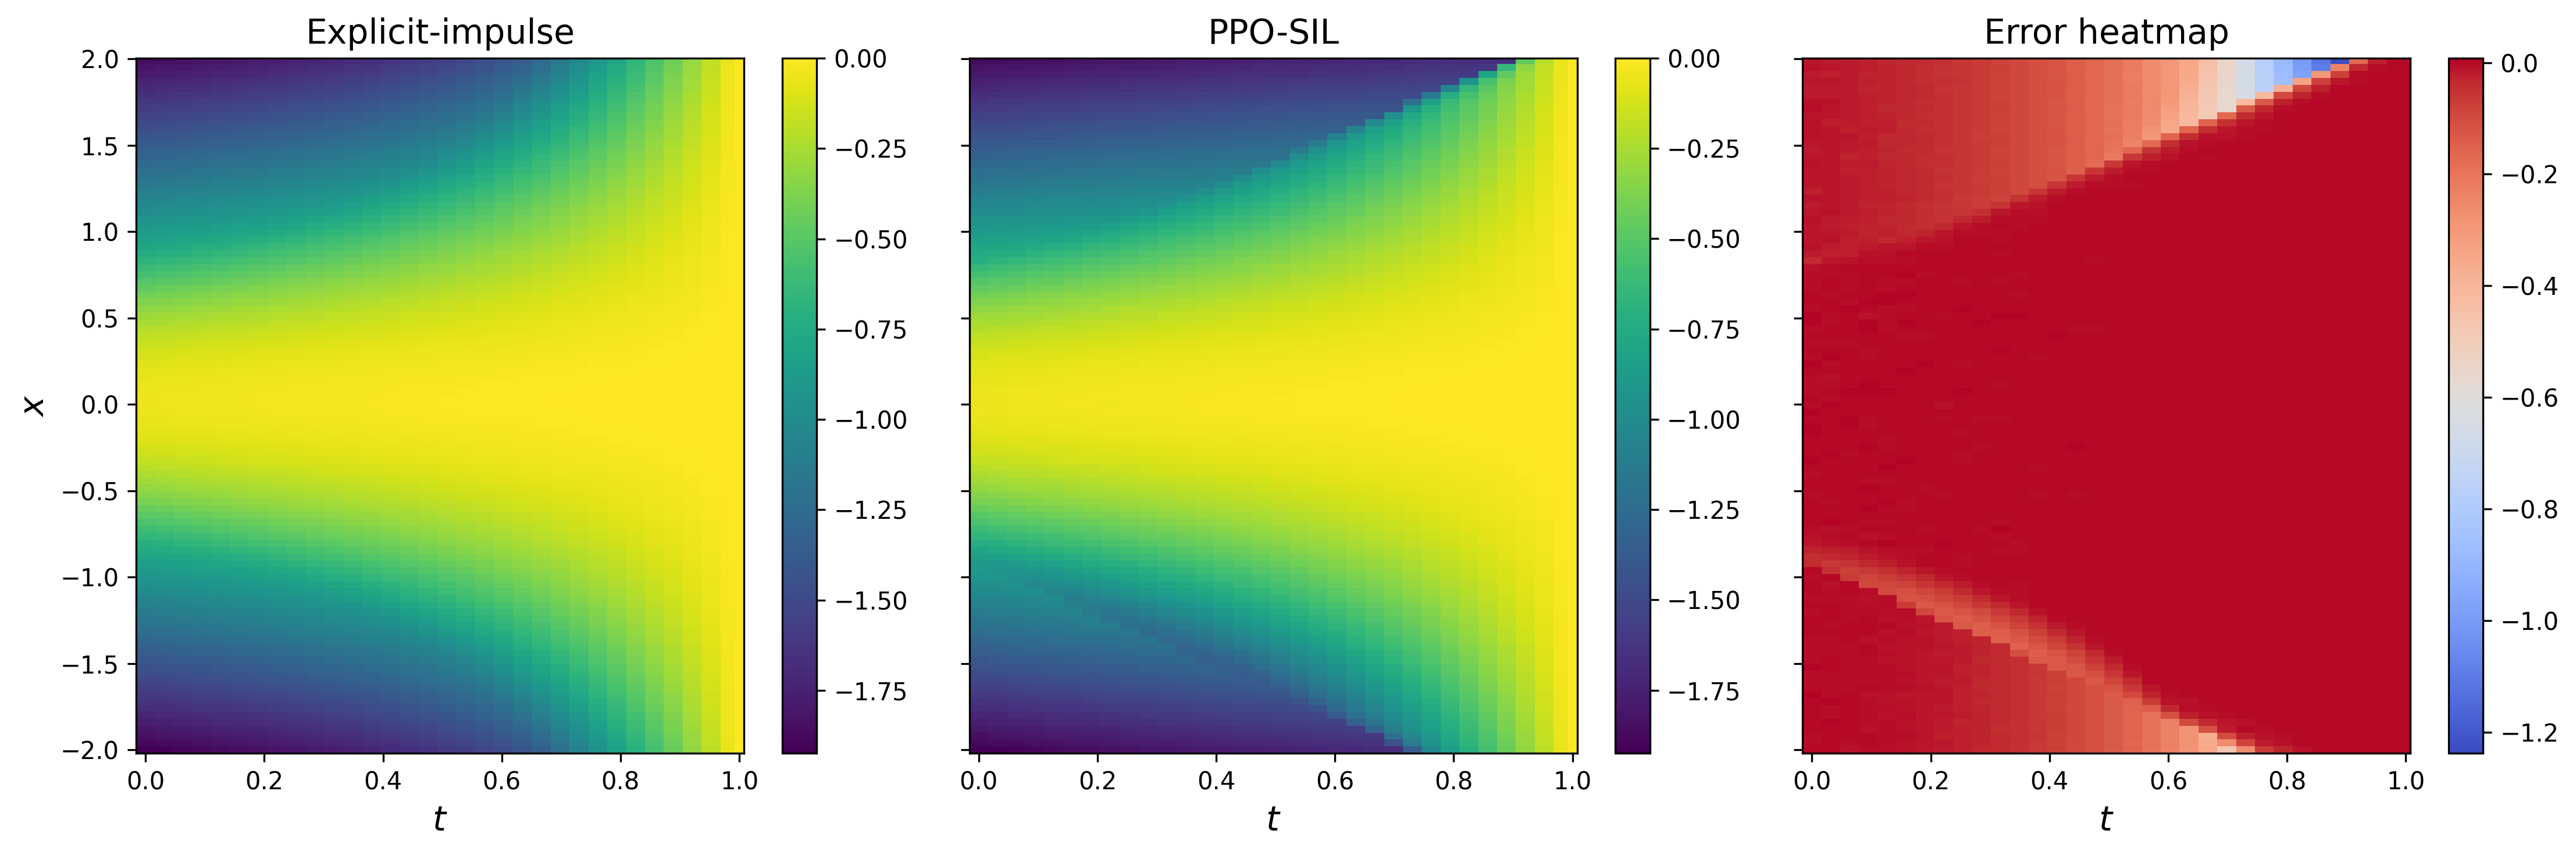
\includegraphics[width=\textwidth]{Plots/FEX/PPO_Error_heatmap.png}
    \caption{Error heatmap of the PPO-SIL algorithm}
    \label{fig: PPO vs FD error plot}
\end{figure}

When it comes to training time, the PPO–SIL model with specifications found in Table \ref{tab: PPO training parameters} needs around 24 minutes, which is significantly less than the DDQN algorithm. However, the explicit‑impulse scheme remains a faster alternative in this particular problem.

In general, the PPO-SIL algorithm approximates the value function well enough for comparison purposes. It captures the continuation region, the affine intervention tails, the time evolution of the value surface, and the approximate free boundary structure. The error heatmap and three-dimensional plot show that the approximation is less reliable near the free boundary and in under-sampled regions of the state space. However, rather than being an issue of the algorithm itself, these errors are mostly caused by the simulation-based nature of the method. Hence, this issue can most likely be addressed by over-sampling the state variable in certain regions. 